\subsection{Statistical analyses including systematics}
\label{lab:Syst_stat}


\subsubsection{ Profiled $\chi^{2}$ with the spurious signal uncertainty}

We can include a spurious sisgnal uncertainty, $s$ to the 
$\chi^{2} = \sum \left(\frac{y_{i} - f_{i}(\mu)}{\sigma_{i}}\right)^{2}$ fit by replacing 
$f(\mu)$ with $F(\mu, \beta*s)$. Where $\beta$ is a nuissance parameter coinstrained by a 
normal Gaussian $N(0,1)$, and $s$ is the size of spurious signal uncertainty. We consider spurious singal
uncertainty is symmetric. For the siganl shpape $d_{u}^{X,Z}$ 
we can write $F(\mu, \beta*s)$ as
 $F_{d,u}^{X,Z}(\mu, \beta*s_{u}^{X,Z}) = 1+(\mu+\beta*s)*(6.28069*cos(x)-41.0569*sin(x))$.
 Then the total $\chi^{2}$ is
  $\chi^{2} = \sum \left(\frac{y_{i} - F_{u,i}^{X,Z}(\mu, \beta*s)}{\sigma_{i}}\right)^{2} + \beta^{2}$.
  Where $i$ is bin index, the $\beta^{2}$ is due to the normal Gaussian constaint of $\beta$.


The figure~\ref{fig:real_data_scrambled_Spurious_signal} shows fit results from profiled $\chi^{2}$ 
with a spurious signal uncertainty $s_{u}^{X,Z} = 3.01e-06$. In the left plot,
 we fit a scrabked dataset. In the right plot, we fit a singal injected toy dataset. In both case, including 
 spurious signal uncertainty enlargened the final fit uncertainty by 
 29\% (28\% for the singal injected toy dataset). 
 The figure~\ref{fig:signal_injected_toy_single_dataset} show the signal injected toy dataset.
 The injected singal amplitude is $\sigma_{LIV}/\sigma_{SM}=0.0009$.


\begin{figure}[ht]
    \centering
    
\includegraphics[width=0.45\textwidth]{figs/partially_unblinded_results/profile_chi2_shape_sys_du_XZ.pdf}
    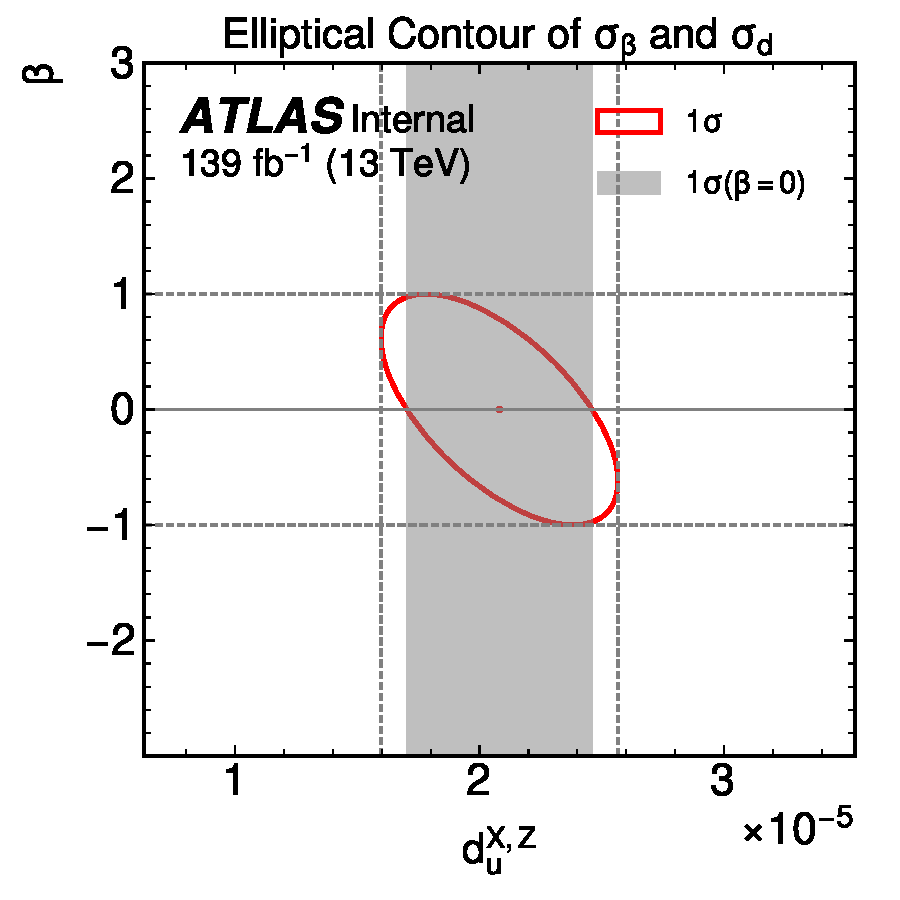
\includegraphics[width=0.45\textwidth]{figs/partially_unblinded_results/profile_chi2_shape_sys_du_XZ_sig0009.pdf}
    
    \caption{Combined fit results of profiled $\chi^{2}$ fit, which includes the spurious
     signal uncertainty as a nuisance parameter $\beta$. The left plot is the result 
     from one of the scrambled datasets. The right plot is a signal-injected toy dataset
      with strength $\sigma_{LIV}/\sigma_{SM}=0.0009$; the signal model is $d_{u}^{X,Z}$. 
    The grey band is the 68\% uncertainty band without spurious signal. The fit uncertainty
     is 29\%(28\% for the toy) larger when we add the spurious signal uncertainty to the fit.}
    \label{fig:real_data_scrambled_Spurious_signal}
\end{figure}
    
    
\begin{figure}[ht]
    \centering
    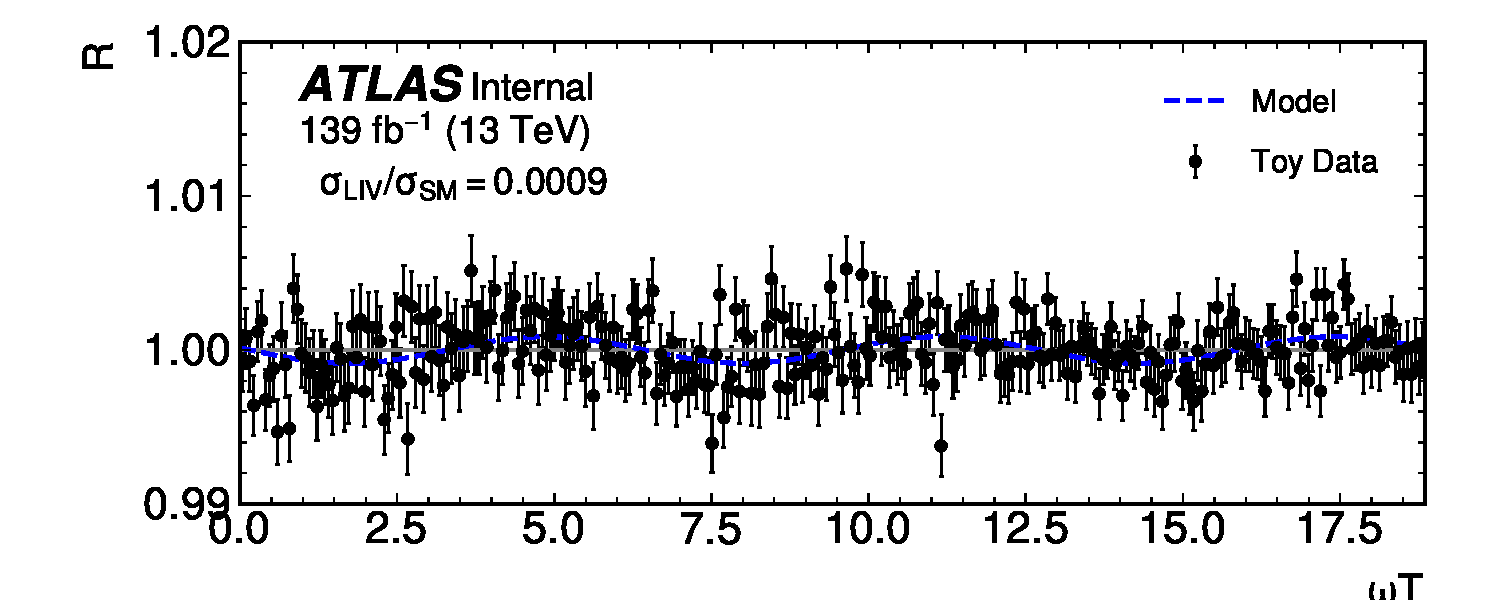
\includegraphics[width=0.90\textwidth]{figs/partially_unblinded_results/profile_chi2_toy_du_XZ_postfit_sig0009.pdf}
    
    \caption{The signal-injected combined toy dataset with signal amplitude
     $\sigma_{LIV}/\sigma_{SM}=0.0009$ and  $d_{u}^{X,Z}$ model (post-fit).
      The blue line is the signal shape after the combined fit. The  error
       bars on the data points are statistical errors.}
    \label{fig:signal_injected_toy_single_dataset}
\end{figure}





\subsection{Summary of results}
\label{lab:Syst_result}
